\chapter{Architetture Parallele}

Per aumentare ancora di più le prestazioni, se è già stato applicato tutto ciò descritto in precedenza, si deve ricorrere a un'architettura dotata di più unità computazionali in modo da avere un \fancyglitter{parallelismo esplicito}. 

\nt{Preso in considerazione il fatto che i programmi debbano andare riscritti per girare su più core.}

\section{I Problemi del Parallelismo Esplicito}

Tuttavia, (eccetto che in casi molto molto particolari) l’incremento di
prestazioni (il cosiddetto \fancyglitter{speed-up}) che si può ottenere usando più
CPU su cui far girare in parallelo i vari programmi è meno che
lineare rispetto al numero di CPU disponibili. Principalmente perché i programmi che girano in parallelo dovranno sincronizzarsi tra loro. Consideriamo il comando "gcc main.c function1.c function2.c -o output". Supponiamo che, lanciando il programma su una macchina monoprocessore ci vogliano 7 secondi: 

\begin{itemize}
  \item 3 secondi per compilare main.c 
  \item 2 secondi per compilare function1.c 
  \item 1 secondo per compilare function2.c 
  \item 1 secondo per linkare gli oggetti. 
\end{itemize}

\paragraph{}
Con 3 CPU a disposizione i tre sorgenti possono essere compilati in parallelo, ma l'operazione di linking può essere eseguita solo dopo che tutti e tre gli oggetti sono stati generati (quindi dopo 3 secondi). In questo modo il tempo si riduce da 7 a 4 secondi con uno speed-up di 1.75 pur avendo usato 3 processori.
\begin{figure}[h]
    \centering
    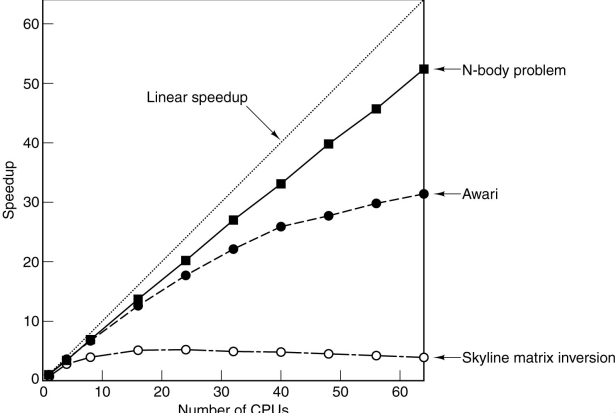
\includegraphics[width=0.3\textwidth]{04-ArchitettureParallele/speed-up.png}
    \caption{Speed-up di alcuni problemi computazionali.}
\end{figure}
\pagebreak
\begin{figure}[!h]
    \centering
    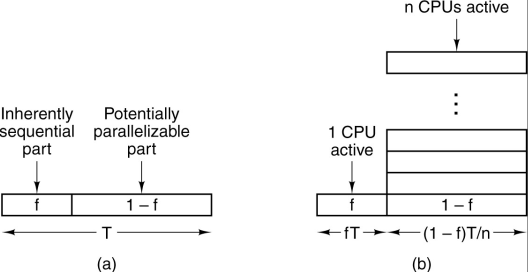
\includegraphics[scale=0.7]{04-ArchitettureParallele/Parallelizzazione limiti.png}
    \caption{Sia P un programma che gira in tempo T su una CPU, con f = la
frazione di T dovuta a codice sequenziale, e (1-f) la frazione di T
dovuta a codice parallelizzabile.}
\end{figure}

\nt{Il tempo di esecuzione dovuto alla parte parallelizzabile, passa
da (1-f)T a (1-f)T/n se sono disponibili n processori. Questa è nota come \fancyglitter{legge di Amdahl}}

\begin{figure}[h]
    \centering
    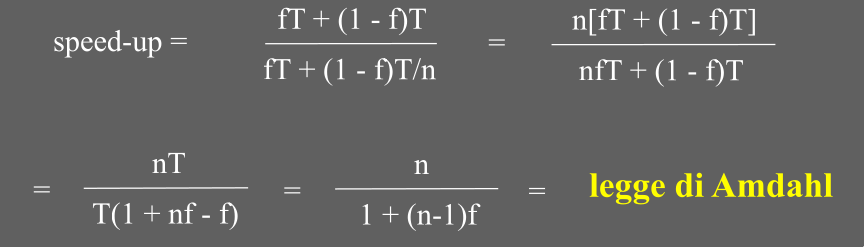
\includegraphics[scale=0.5]{04-ArchitettureParallele/Legge di Amdahl.png}
    \caption{La legge di Amdahl.}
\end{figure}

\begin{itemize}
  \item Se si vuole ottenere uno speed-up perfetto, pari al numero di CPU usate, f deve valere 0, ma ciò è impossibile. 
  \item Spesso il miglioramento è sub-lineare.
\end{itemize}

\paragraph{I problemi del parallismo esplicito sono generalmente due:}

\begin{enumerate}
  \item La quantità limitata di parallelismo nel codice dei programmi (problema software). 
  \item Gli elevati costi delle comunicazioni tra processori e memoria (problema hardware).
\end{enumerate}

\nt{Per molte applicazioni avere uno speed-up, seppur limitato, è comunque accettabile, perché: 
\begin{itemize}
  \item La presenza di più processori aumentà l'affidabilità del sistema. 
  \item Servizi che per loro natura sono forniti su ampia scala geografica,
devono essere implementati con una architettura distribuita. Se il
sistema fosse centralizzato in un unico nodo, l’accesso di tutte le
richieste a quest’unico nodo costituirebbe probabilmente un collo
di bottiglia in grado di rallentare enormemente il servizio fornito.
\end{itemize}
}

\paragraph{Ci sono tre tipi di architetture parallele esplicite:}

\begin{itemize}
  \item Multi-threading (a). 
  \item Sistemi a memoria condivisa (b, c). 
  \item Sistemi a memoria distribuita (d, e).
\end{itemize}

\begin{figure}[h]
    \centering
    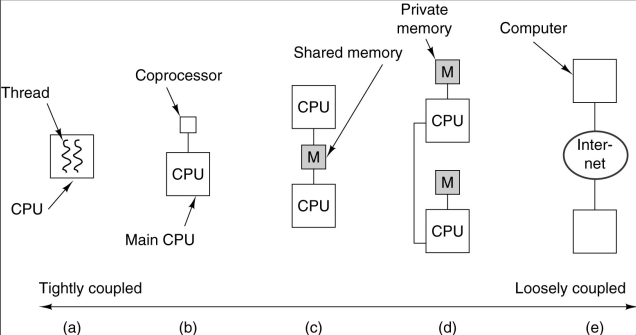
\includegraphics[scale=0.5]{04-ArchitettureParallele/PE.png}
    \caption{Vari tipi di architetture esplicitamente parallele.}
\end{figure}

\section{Multi-Threading}

\subsection{Introduzione}

\dfn{Architettura Multi-Threaded}{
  Una CPU multi-threaded è una architettura parallela un po’
particolare, in quanto il multi-threading è realizzato con un’unica
CPU (sempre single core), ma porta il programmatore
a concepire e sviluppare le sue applicazioni come formate da un
insieme di programmi che possono essere eseguiti in parallelo:
i thread.
}

\nt{Se questi programmi vengono fatti girare su una CPU che supporta il multi-threading ne sfrutteranno le caratteristiche architetturali.}

\paragraph{}

L’idea del multi-threading nasce dalla constatazione di un problema
di fondo presente in qualsiasi CPU pipelined: un cache miss
produce una “lunga” attesa necessaria per recuperare l’informazione
mancante in RAM. Se non c’è un’altra istruzione indipendente da poter eseguire,
o se non è implementato lo scheduling dinamico della pipeline,
la pipeline va in stall. Una soluzione per non sprecare inutilmente cicli di clock in attesa
del dato mancante è il multithreading: permettere alla CPU di
gestire più peer-thread allo stesso tempo: se un thread è bloccato
la CPU ha ancora la possibilità di eseguire istruzioni di un altro
thread, in modo da tenere le varie unità funzionali comunque
occupate.

\clm{}{}{
  \begin{itemize}
    \item Per implementare il multithreading, la CPU deve poter gestire lo
stato della computazione di ogni singolo thread. 
\item Ci deve essere un Program Counter (PC) e un set di registri separato per ciascun thread.  
\item Il thread switch deve essere più efficiente del process switch.
  \end{itemize}
}

\subsection{Tipi di Multi-Threading}

\paragraph{Esistono due tecniche di base per il multi-threading:}

\begin{itemize}
  \item \fancyglitter{Fine-grained multi-threading}. 
  \item \fancyglitter{Coarse-grained multi-threading}.
\end{itemize}

\dfn{Fine-grained Multi-Threading}{
  Lo switching tra i vari peer-thread
avviene ad ogni istruzione, indipendentemente dal fatto che
l’istruzione del thread in esecuzione abbia generato un cache miss.

Lo \newfancyglitter{scheduling} tra i vari peer-thread avviene secondo una politica round robin e la CPU deve essere in grado di effettuare lo switch praticamente senza overhead (che sarebbe inaccettabile).
}
\nt{Se vi è un numero sufficiente di peer-thread, è possibile che ve ne
sia sempre almeno uno non in stall, e la CPU può essere mantenuta
sempre attiva.}

\clm{}{}{
\begin{itemize}
  \item Lo stalling della CPU può anche essere dovuto a una dipendenza o a un branch, poiché l'ILP dinamico non può sempre evitarlo.
  \item Invece, con il Fine-grained multithreading, in un'architettura pipelined, se: 
    \begin{itemize}
      \item La pipeline ha $k$ stage. 
      \item Ci sono almeno $k$ peer-thread da eseguire. 
      \item La CPU esegue lo switch tra thread a ogni ciclo di clock.
    \end{itemize}
  \item Non ci può essere mai più di un'istruzione per thread nella pipeline in un dato istante, le dipendenze sui dati vengono risolte automaticamente e la pipeline non va mai in stall (se un cache miss può essere gestito in un numero di cicli di clock inferiore o uguale al numero di thread in esecuzione).
\end{itemize}
}

\begin{figure}[h]
    \centering
    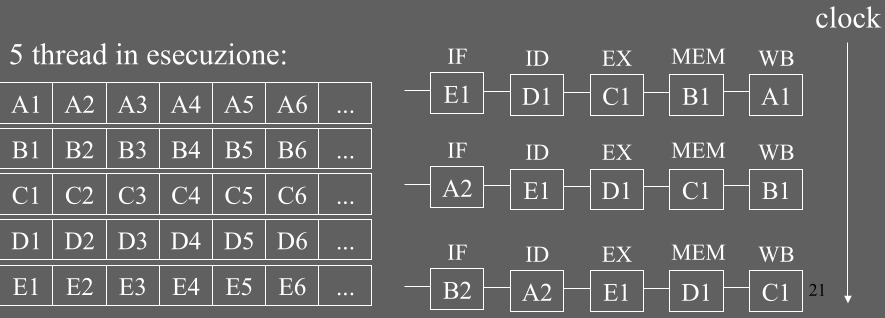
\includegraphics[scale=0.5]{04-ArchitettureParallele/fine.png}
    \caption{Fine-grained multithreading in una CPU con pipeline
     a 5 stadi.}
\end{figure}

\nt{Lo scheduling Fine-grained fa si che un thread venga rallentato anche quando potrebbe proseguire l'esecuzione perché non sta generando alcuno stall (per via del fatto che vada eseguito un context switch a ogni istruzione). Inoltre potrebbero esserci meno thread che stage della pipeline, per cui non è facile mantenere la CPU sempre occupata.}

\dfn{Coarse-grained Multi-Threading}{
Lo switch avviene solo quando il
thread in esecuzione genera uno stall, provocando così lo spreco di
un ciclo di clock.

Viene effettuato lo switch a un altro thread. Quando anche questo genererà uno stall verrà schedulato un terzo thread (o eventualmente si tornerà al primo) e così via. 
}

\nt{Questo approccio spreca potenzialmente più cicli di clock rispetto al Fine-grained, perché comunque lo switch avviene solo se si è verificato uno stall. Ma se ci sono pochi thread attivi questi possono essere sufficienti per tenere la CPU occupata.}

\paragraph{Fine-grained vs. Coarse-grained:}

\begin{itemize}
  \item Non è pensabile che lo switch tra thread possa avvenire senza perdite di tempo.
  \item Se le istruzioni dei vari thread non generano stall molto frequentemente uno scheduling Coarse-grained è più vantaggioso (perché il Fine-grained, ogni ciclo di clock, paga un overhead limitato, ma non nullo).
  \item Fine-grained $\rightarrow$ Sistema operativo time-sharing. 
  \item Coarse-grained $\rightarrow$ Sistema operativo multitasking.
\end{itemize}

\dfn{Medium-grained Multi-Threading}{
  Una via di mezzo tra il fine- e il
coarse- grained multithreading consiste nell’eseguire lo switch tra
thread solo quando quello in esecuzione sta per eseguire una
istruzione che potrebbe generare uno stall di lunga durata,
come ad esempio una load (che potrebbe richiedere un dato non
in cache), o un branch (perché anche l'istruzione nel caso il branch venisse preso potrebbe non trovarsi nelle cache L1, L2, L3).

L'istruzione viene avviata, ma il processore esegue in ogni caso lo switch a un altro thread.
}

\nt{In questo modo non si spreca neanche il ciclo di clock dovuto all'eventuale stall dell'istruzione eseguita (come accade nel Coarse-grained).}

\qs{}{Ma come si fa a sapere a quale thread appartiene una qualsiasi
istruzione nella pipeline?}

\begin{itemize}
  \item Nel caso del Fine-grained Multi-Threading l'unico modo è di attaccare un \fancyglitter{thread identifier} a ogni istruzione. Per esempio l'ID univoco associato a quel thread all'interno dell'insieme di peer-thread a cui appartiene. 
  \item Nel caso del Coarse-grained Multi-Threading si può adottare la stessa soluzione oppure si può anche svuotare la pipeline a ogni thread switch (in questo modo le istruzioni di un solo thread alla volta sono nella pipeline e quello sa sempre a quale thread appartengono). 
\end{itemize}

\nt{Ciò ha senso solo se lo switch avviene a intervalli molto maggiori del tempo necessario a svuotare la pipeline. Inoltre, le istruzioni dei vari thread, devono essere, per quanto possibile, tutte contemporaneamente nella cache delle istruzioni, altrimenti ogni context switch tra thread produce un cache miss e si perde qualsiasi vantaggio nell'utilizzare i thread.}

\subsection{Simultaneous Multi-Threading}

Le moderne \fancyglitter{architetture superscalari}, multiple issue e a scheduling dinamico della pipeline danno la possibilità di sfruttare contemporaneamente il parallismo insito nelle istruzioni di un programma (ILP) con il parallelismo insito in un insieme di peer-threads: il Thread Level Parallelism (TLP). 

\begin{center}
  \fancyglitter{ILP + TLP = SMT (Simultaneous Multi-Threading)}
\end{center}

\nt{Le ragioni per implementare SMT risiedono nell'osservazione che le moderne CPU multiple issue hanno più unità funzionali di quante siamo mediamente sfruttabili dal singolo thread in esecuzione. 

Sfruttando il register renaming e lo scheduling dinamico istruzioni appartenenti a thread diversi possono essere eseguite insieme.
}

\begin{figure}[h]
    \centering
    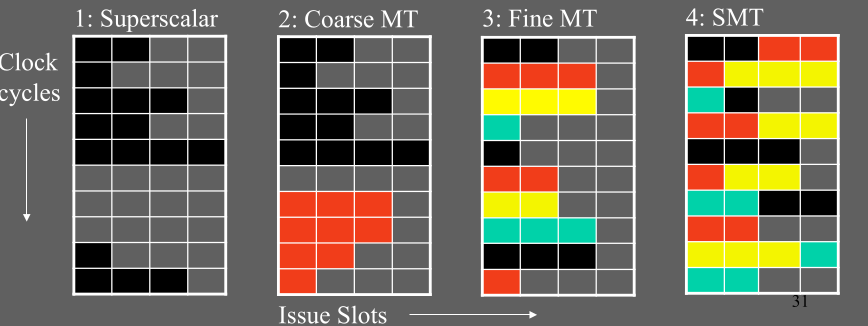
\includegraphics[scale=0.5]{04-ArchitettureParallele/SMT.png}
    \caption{Confronto tra processori.}
\end{figure}

\clm{}{}{
  \begin{itemize}
    \item Anche nel SMT non si riesce sempre ad avviare il massimo numero possibile di istruzioni per ciclo di clock a causa del numero limitato di unità funzionali e di stazioni di prenotazione disponibili, della capacità della cache di istruzioni di fornire le istruzioni dei vari thread e del numero di thread presenti. 
    \item SMT può essere adeguatamente supportato solo se sono disponibili registri rinominabili in abbondanza. 
    \item Nel caso di una CPU che supporti la ridenominazione sarà importante avere un ROB distinto per ogni thread in modo da gestire in maniera indipendente i commit.
  \end{itemize}
}

\subsubsection{Il Multi-Threading Intel}

\dfn{Hyperthreading}{
  Viene supportata l’esecuzione di due thread in modalità SMT.
}

\clm{}{}{
  \begin{itemize}
    \item Dal punto di vista del Sistema Operativo, una CPU multithreaded
è vista come due CPU che condividono cache e RAM: dunque due
applicazioni che condividono lo stesso spazio di indirizzamento,
possono essere eseguite in parallelo nei due thread. 
\item Siccome due thread possono usare contemporaneamente la CPU,
occorre adottare delle strategie per fare in modo che entrambi i
thread possano utilizzare le varie risorse della CPU.
  \end{itemize}
}

\paragraph{\fancyglitter{Ci sono 4 strategie ideate da Intel:}}

\begin{itemize}
  \item \fancyglitter{Risorse duplicate:} quelle necessarie a gestire l'esecuzione dei due thread (due program counter e due banchi di registri separati). 
  \item \fancyglitter{Risorse partizionate equamente tra i due thread:} la coda delle microistruzioni e il ROB. 
  \item \fancyglitter{Risorse condivise dinamicamente:} un thread può occupare quante linee di cache vuole, eventualmente rallentando l'altro thread. 
  \item \fancyglitter{Risorse condivise dinamicamente:} lo scheduler che invia le uops alle varie stazioni di prenotazione. 
\end{itemize}

\begin{figure}[h]
    \centering
    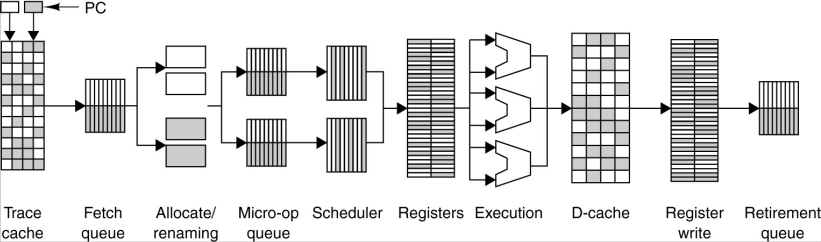
\includegraphics[scale=0.5]{04-ArchitettureParallele/Intel.png}
    \caption{Risorse in una CPU Intel.}
\end{figure}

\paragraph{Brevi note storiche:}

\begin{itemize}
  \item Intel abbandona la tecnologia Hyperthreading nel passaggio ai nuovi processori dual core (non supportavano il multithreading). 
  \item L'Hyperthreading è stato reintrodotto a partire dal 2008 con l'architettura Nehalem. 
  \item IBM Power 7 (2010) implementò SMT con 4 thread contemporaneamente attivi. 
  \item I processori UltraSPARK, da T2 in poi, supportano il Fine-grained multithreading con 8 thread per core. L'UltraSPARK T1 solo 4 thread per core.
\end{itemize}

\section{Multiprocessori a Memoria Condivisa}

\subsection{Introduzione}

\dfn{Multiprocessore}{
  Un \newfancyglitter{multiprocessore} è un'architettura con più CPU che condividono la stessa memoria primaria. 
 }
 \subsubsection{}
 In un sistema multiprocessore tutti i processi che girano sulle varie CPU condividono un unico spazio di indirizzamento logico, mappato su una memoria fisica che può però anche essere distribuita tra i vari banchi di memoria in modi diversi. Ogni processo può leggere e scrivere un dato in memoria specificando un indirizzo usato da LOAD e STORE, e la comunicazione tra processi avviene attraverso la memoria condivisa.


 \nt{È responsabilità dell’hardware del sistema fare in modo che tutte
le CPU possano vedere e usare la stessa memoria principale.}

\begin{figure}[h]
    \centering
    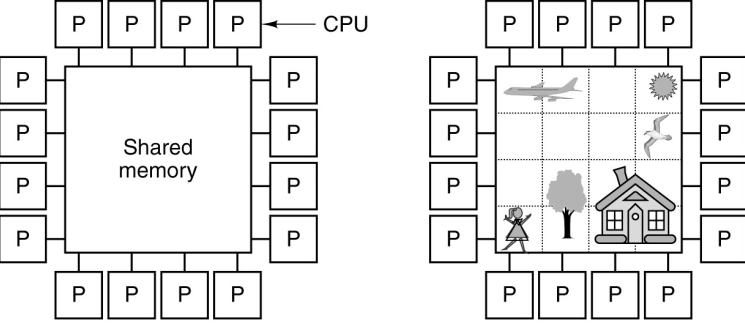
\includegraphics[scale=0.5]{04-ArchitettureParallele/Multi.png}
    \caption{Schema di base di un multiprocessore.}
\end{figure}

\clm{}{}{
  \begin{itemize}
    \item Siccome tutte le CPU vedono lo stesso spazio di indirizzamento,
è sufficiente una copia del sistema operativo. 
\item Quando un processo termina o va in wait per qualche ragione, il
S.O. può cercare nella coda di ready un altro processo a cui dare la
CPU idle. 
\item Al contrario, nei sistemi a memoria non condivisa, ogni CPU deve
far girare la propria copia del sistema operativo, e i processi
possono comunicare solo attraverso lo scambio di messaggi. 
\item Il problema di fondo dei sistemi multiprocessore a memoria
condivisa è la memoria stessa, che è difficile da far funzionare
in maniera efficiente quanto più è alto il numero dei processori
coinvolti.
  \end{itemize}
}

\qs{}{Come funzionano i sistemi multiprocessore?}

\begin{itemize}
  \item Tutti i moderni SO (Windows, Solaris, Linux, MacOS) prevedono in
particolare la cosiddetta multielaborazione simmetrica (symmetric
multiprocessing, SMP), in cui (tralsciando un po’ di cose) uno
scheduler gira su ciascun processore. 
\item I processi “ready to run” possono essere inseriti in un’unica coda,
vista da ciascun scheduler, oppure vi può essere una coda “ready to
run” separata per ciascun scheduler/processore. 
\item Quando lo scheduler di un processore si attiva, sceglie uno dei
processi “ready to run” e lo manda in esecuzione sul proprio
processore.
\item Un aspetto importante dei sistemi multiprocessore è il bilanciamento
del carico.
\item Non ha infatti senso avere un sistema con più CPU se poi i vari
processi da eseguire non sono distribuiti più o meno omogeneamente
tra i vari processori. 
\item Nel caso di un’unica coda ready to run, il bilanciamento del carico
è solitamente automatico: quando un processore è inattivo, il suo
scheduler prenderà un processo dalla coda comune e lo manderà in
esecuzione su quel processore.
\item I SO moderni predisposti per l’SMP usano però spesso una coda
separata per ciascun processore in modo da non doversi sincronizzare
per accedere all’unica coda di ready quando devono inserire o
prelevare un processo dalla coda. Esiste allora un esplicito meccanismo di bilanciamento del carico
che può prendere un processo in attesa sulla coda di un processore
sovraccarico e spostarlo nella coda di un processore scarico\footnote{Per esempio, in Linux SMP meccanismo di bilanciamento del carico
si attiva ogni 200 millisecondi, e ogni qualvolta si svuota la coda di
un processore.}.
\end{itemize}

\subsection{Tipi di Architetture Multiprocessore}

Esistono sostanzialmente due classi di architetture multiprocessore: 

\begin{itemize}
  \item \fancyglitter{UMA}. 
  \item \fancyglitter{NUMA}.
\end{itemize}

\nt{Una terza classe, detta \fancyglitter{COMA} (Cache Only Memory Architecture), sebbene teoricamente promettente non è stata mai implementata in maniera soddisfacente.}

\dfn{UMA}{
  Uniform Memory Access (UMA) è un tipo di architettura in cui tutti i processori condividono un'unica memoria primaria centralizzata e quindi ogni CPU ha lo stesso tempo di accesso alla memoria. 
}

\nt{Questi sistemi vengono anche chiamati SMP (Symmetric Shared-Memory Multiprocessor)}

\begin{figure}[h]
    \centering
    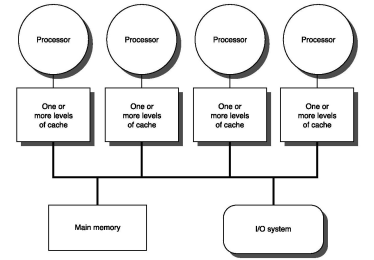
\includegraphics[scale=0.8]{04-ArchitettureParallele/UMA.png}
    \caption{Schema UMA.}
\end{figure}

\dfn{NUMA}{ 
Non Uniform Memory Access (NUMA) è un tipo di architettura in cui la memoria fisica è distribuita tra le varie CPU e quindi i tempi di accesso ai dati variano a seconda che siano nella RAM locale o in una remota.
}

\nt{Questi sistemi vengono anche chiamati DSM (Distribuited Shared-Memory)}

\begin{figure}[h]
    \centering
    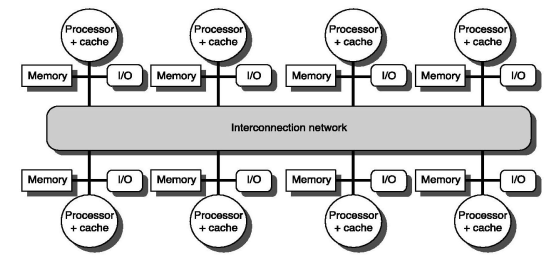
\includegraphics[scale=0.8]{04-ArchitettureParallele/NUMA.png}
    \caption{Schema NUMA.}
\end{figure}

















